\chapter{坐标几何}
\label{ch:Coordinate Geometry}
坐标几何学是代数学和几何学两者共同孕育出来的儿子。
当笛卡尔发明了坐标轴系统之后,几何学中的平面上的点,可以用两个坐标轴的数值进行确定;几何学中的直线与线性函数的的图像就变成了同一个事物,可以用含有$x$,$y$的代数式进行表示。于是坐标几何学就诞生了。

也成为了现在\href{https://www.autodesk.com}{AutoCad},Blender,\href{https://www.geogebra.org}{Geogebra}这些软件的基石。

\section*{学习目标}
\begin{todolist}
 \item 根据已知信息求算直线的表达式
 \item 掌握表示直线的几种形式,包括\gls{xjs},\gls{dxs}以及\gls{ybs}
 \item 理解并运用\gls{bzfc}
 \item 利用代数运算求解直线和圆有关的问题
 \item 理解任意图形与其代数表达式的等价关系
 \item 利用图像的交点求算方程的解
\end{todolist}
\clearpage

\section{直线}
\label{sec:Straight Line}
直线是除了点之外,最简单的几何图形,直线的表达式必定可以用
\[
	y=mx+c
\]
进行表示的。而且由于两点确定一条直线,因此求算坐标系中直线的表达式仅需要提供两个点就可以了。\gls{slope}的求算通过:
\[
	m=\frac{y_2-y_1}{x_2-x_1}
\]

\gls{jj}则可以带入到任何一个点的横纵坐标,进而确定。

\begin{TaskBox}
Find the slope-intercept form a line passnig through the point $(2,5)$ and $(3,4)$.
\end{TaskBox}

\subsection*{点斜式}
\label{subsec:Point Slope Form}
如果给定的信息是斜率和一个点的坐标的话,其实我们有更加简洁的方式去定义这条线。比如在上一条Task当中,该直线的斜率为$-1$,如果再已知该直线通过一个点$(3,4)$的话,利用斜率的定义:
\begin{align}
 \notag m=-1 &=\frac{y-4}{x-3}\\ %编号和引用参考的问题
  y-4 &=-1(x-3)
\end{align}

将直线所通过的点的横纵坐标,以及该直线的斜率全部表述出来的形式被称之为\gls{dxs}。具有如下的形式:
\[
	y-y_0 = m(x-x_0)
\]
其中,$m$是斜率,$(x_0,y_0)$是直线当中某一个点的具体坐标。

\begin{TaskBox}
思考,$y=m(x)+c$ 如何修改为点斜式,使其通过的点为$y$轴截距
\end{TaskBox}


\subsection*{普通式}
\label{subsec:Standard Form of a line}
在之前的两种形式中,需要某一条直线具有特定的斜率。但是,当一条完全垂直于$x$轴的直线式,无论如何,都无法用上面的两种形式进行表示。因为这样的线是没有斜率的,或者说斜率是underfined。为了能够囊括所有的直线。我们把$x$,$y$都移动到同一侧,得到如下的直线的形式:
\[
	ax+by=c \qquad ax+by+c=0
\]
在这样的表达式中,斜率并没有直接体现出来。但是,这种表达式的好处在于,$x$和$y$之前的系数可以为0。包含了完全水平的直线$by=c$,或者完全垂直的直线$ax=c$,这两种额外的形式。

\begin{TaskBox}
将$y=-x+7$整理为普通式
\end{TaskBox}
\clearpage


\section{圆的标准方程}
\label{sec:Standard Equation of a Cricle}
回顾一下两点间的距离公式:
\[
	d=\sqrt{(x_2-x_1)^2+(y_2-y_1)^2}
\]

再回顾一下圆的定义:\\
到固定点的长度等于固定值的所有的点所形成的几何图形。该固定点称之为圆心,该固定值长度称之为\gls{radius}。

于是,在一个坐标系中,假设$(x,y)$是圆上任意一点,$(a,b)$为圆心,$r$为该圆的半径。那么$x$,$y$必定满足如下的方程
\[
	(x-a)^2+(y-b)^2=r^2
\]
形如这样的表达式的方程被称为\gls{bzfc}。在这种表达式下,圆心坐标和半径就被清楚地罗列出来了。

\begin{figure}[H]
\centering
\includegraphics[width=0.8\textwidth]{rainbow}
\caption{彩虹就是标准的圆形}
\end{figure}

打开该\href{https://www.desmos.com/calculator/nasxcwsa73}{Desmos}演示,查看一道美丽的正圆彩虹。

\begin{TaskBox}
为什么这里不称之为圆的函数,而只能叫做圆的方程?
\end{TaskBox}

\subsection*{圆的一般方程}
\label{subsec:Normal Equation of a circle}
当然,由于二次平方的展开,圆的标准方程也可以展开为普通方程:
\begin{align*}
	(x-a)^2+(y-b)^2 &=r^2\\
	x^2-2ax+a^2+y^2-2by+b^2 &=r^2\\
	x^2+y^2+Ax+By+C&=0
\end{align*}

所以这两者之间要能够互相转化。

\begin{TaskBox}
将$x^2+2x+y^2-4y-3=0$转变为圆的标准方程,并写出该圆的圆心坐标和半径。
\end{TaskBox}

\subsection*{点和圆的位置关系}
\label{subsec:Position of a Point with repsect to a Circle}
当一个点在圆内时,其到圆心的距离必定小于半径,因此沿用标准方程:
\[
	(x-h)^2+(y-k)<r^2
\]
就表示在圆内的所有点。

当一个点在圆外时,其到圆心的距离必定大于半径,继续沿用标准方程:
\[
	(x-h)^2+(y-k)>r^2
\]
就表示在圆外的所有点。
\clearpage


\section{直线与圆的联立}
\label{subsec:Line and Circle}
一条直线和圆会形成相交,相切,以及相离的位置关系。如下图所示:
\begin{figure}[H]
\centering
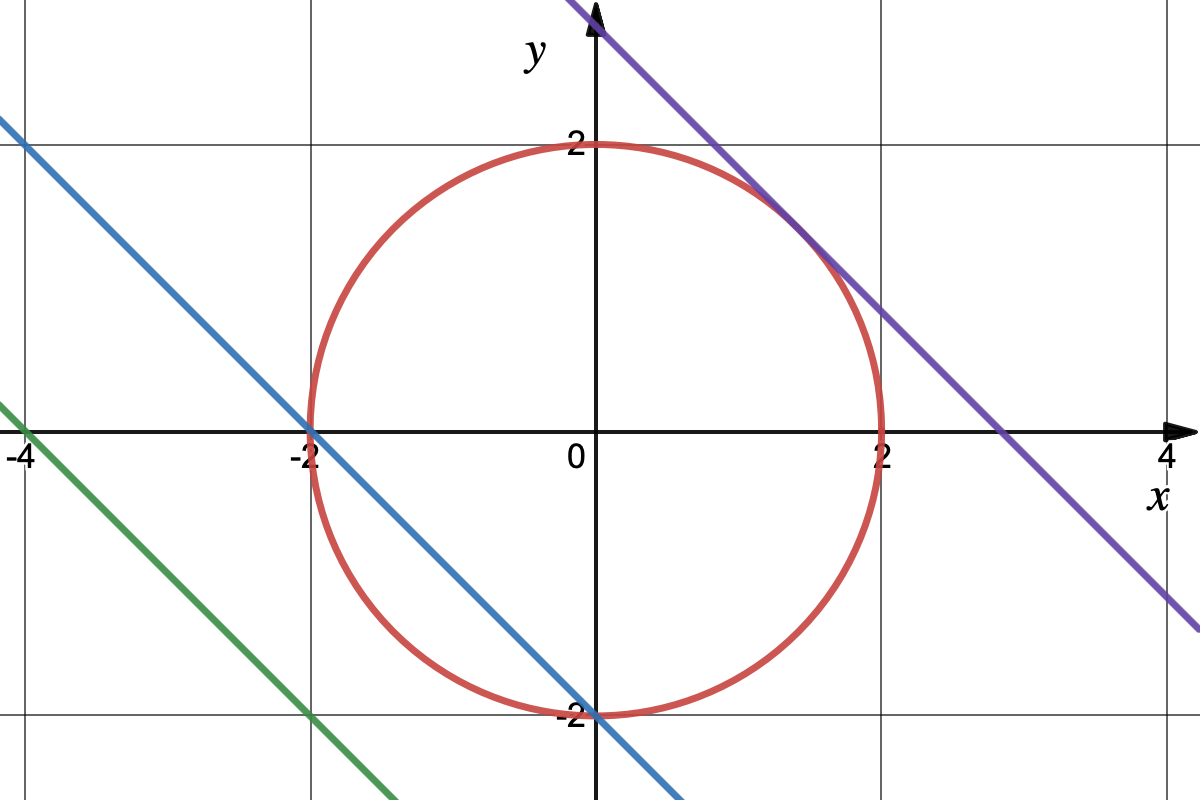
\includegraphics[width=0.8\textwidth]{lineCircle}
\caption{三种不同的圆和直线的关系}
\end{figure}

根据之前所学,由于直线和圆都具有代数表达式,因此将其对应的代数式进行联立得到如下的方程组:
\[
\left\{\begin{matrix}
y=mx+c\\
(x-a)^2+(y-b)^2=r^2
\end{matrix}\right.
\]
该表达式的解就是对应图像的交点。而解决该方程组的固定做法是:

\noindent1.利用$y$和$x$的线性关系,只保留一个变量\\
2.将圆的方程转变为关于$x$或者$y$的一元二次方程\\
3.求解该方程,并将结果带入到线性函数中。确定坐标。

\begin{TaskBox}
证明直线$y=-x+2\sqrt 2$与$x^2+y^2=4$相切,求算其切点
\end{TaskBox}
\clearpage

